\section{Flow architectures}
\label{app:flows-details}

\subsection{Real NVP}

One of the simplest types of flow architectures is the Real-NVP \cite{1605.08803}. 
To keep the Jacobian inverse computation diagonal, we take turns transforming the variables, b/c transforming then the Jacobian becomes block diagonal, transforming the inverse operation from $\mathcal{O}(n^3)$ to $\mathcal{O}(n^2)$ (where $n$ is the dimension of the modelling variables.

To ensure that the matrix stays block diagonal, let each step of the flow $f_{i}$ transform just half of the variable dimensions at a time.
 
Below we show the architecture for a  2 variable flow modelling the variables $m_{hh}$ and $|\cos \Theta^*|$ (where $\Theta^*$ is the polar angle of one of the HCs in the HH rest frame \cite{paper from Rafael}). \Fig{\ref{fig:rnvp-graphic}} shows how we go from a 2d Gaussian density , and each $f_i$ step of the flow allows us to go successively modify the vector $z$ until we recover the HH kinematics.
For example, in the first step of the flow, $f_0$, the first dimension of the flow $z_0$ is transformed with the scale and shift as a function of $z_1$. 
To preserve the bijection, affine transformations are used where the variable being transformed.
The scale and shift values of the affine transformation are allowed to depend on the other (non-transforming) variables and are small NNs to predict.
Since the variables go one-at-a-time, the inverse computation remains tractable, i.e, when $z_1$ is known, it's trivial to solve for $f_0^{-1}$ as $z_0 \rightarrow \left( z_01- t(z_1) \right) / s (z_1)$.

\begin{itemize}
	\item Talk about $f^{-1}$
	\item The s and t are NNs (different for each fi) 
	\item Parameters optimized by maximizing the likelihood of the data $p_y(y)$
	\item Ensure the positivity of $s$ by exponentiating the output of s
\end{itemize}

\begin{figure}[hbt]
    \centering
    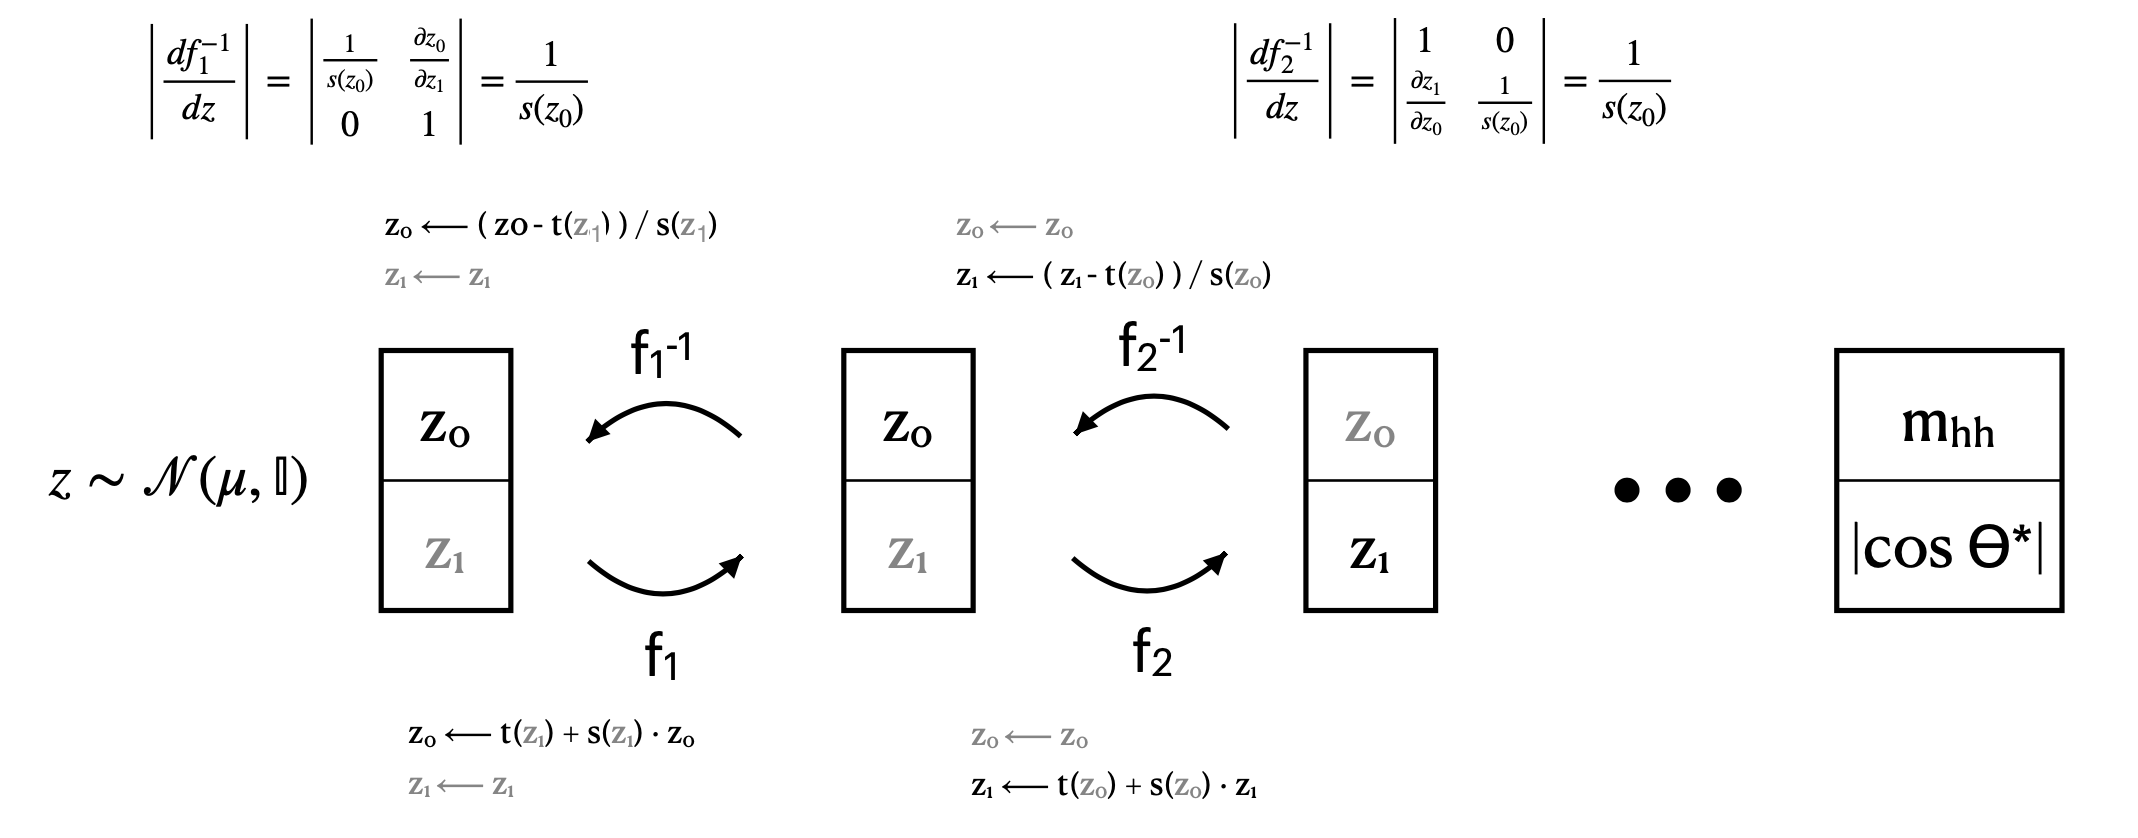
\includegraphics[width=\textwidth]{figures/flows/flow-architectures/Real-NVP-graphic}
    \caption{Graphic for explaining how a Real-NVP works for a 2 variable flow.}
    \label{fig:rnvp-graphic}
\end{figure}

Note - in 2d, both the implementation for Masked Autoregressive Flow (MAF) \cite{MAF} and the Inverse Autoregressive Flow (IAF) \cite{IAF} are identical with Real-NVP. 
But pne of the attractive aspects of the Real-NVP as we. extend to more variables is it is equally fast both for density estimation (i.e, model training) and sampling (or predicting the kinematics distributions), so this is why we show some of our preliminary model optimizations.

To solve the interpolation problem, we want the kinematics to depend on $(m_{h1}),m_{h2})$, which can be done by passing $(m_{h1}),m_{h2})$ as additional variables to the scale and shift networks which still preserves the nice properties of the bijection of each of the flow steps while the Jacobians remain tractable with the modification to the math shown in \Fig{\ref{fig:rnvp-cond}}.

\begin{figure}[hbt]
    \centering
    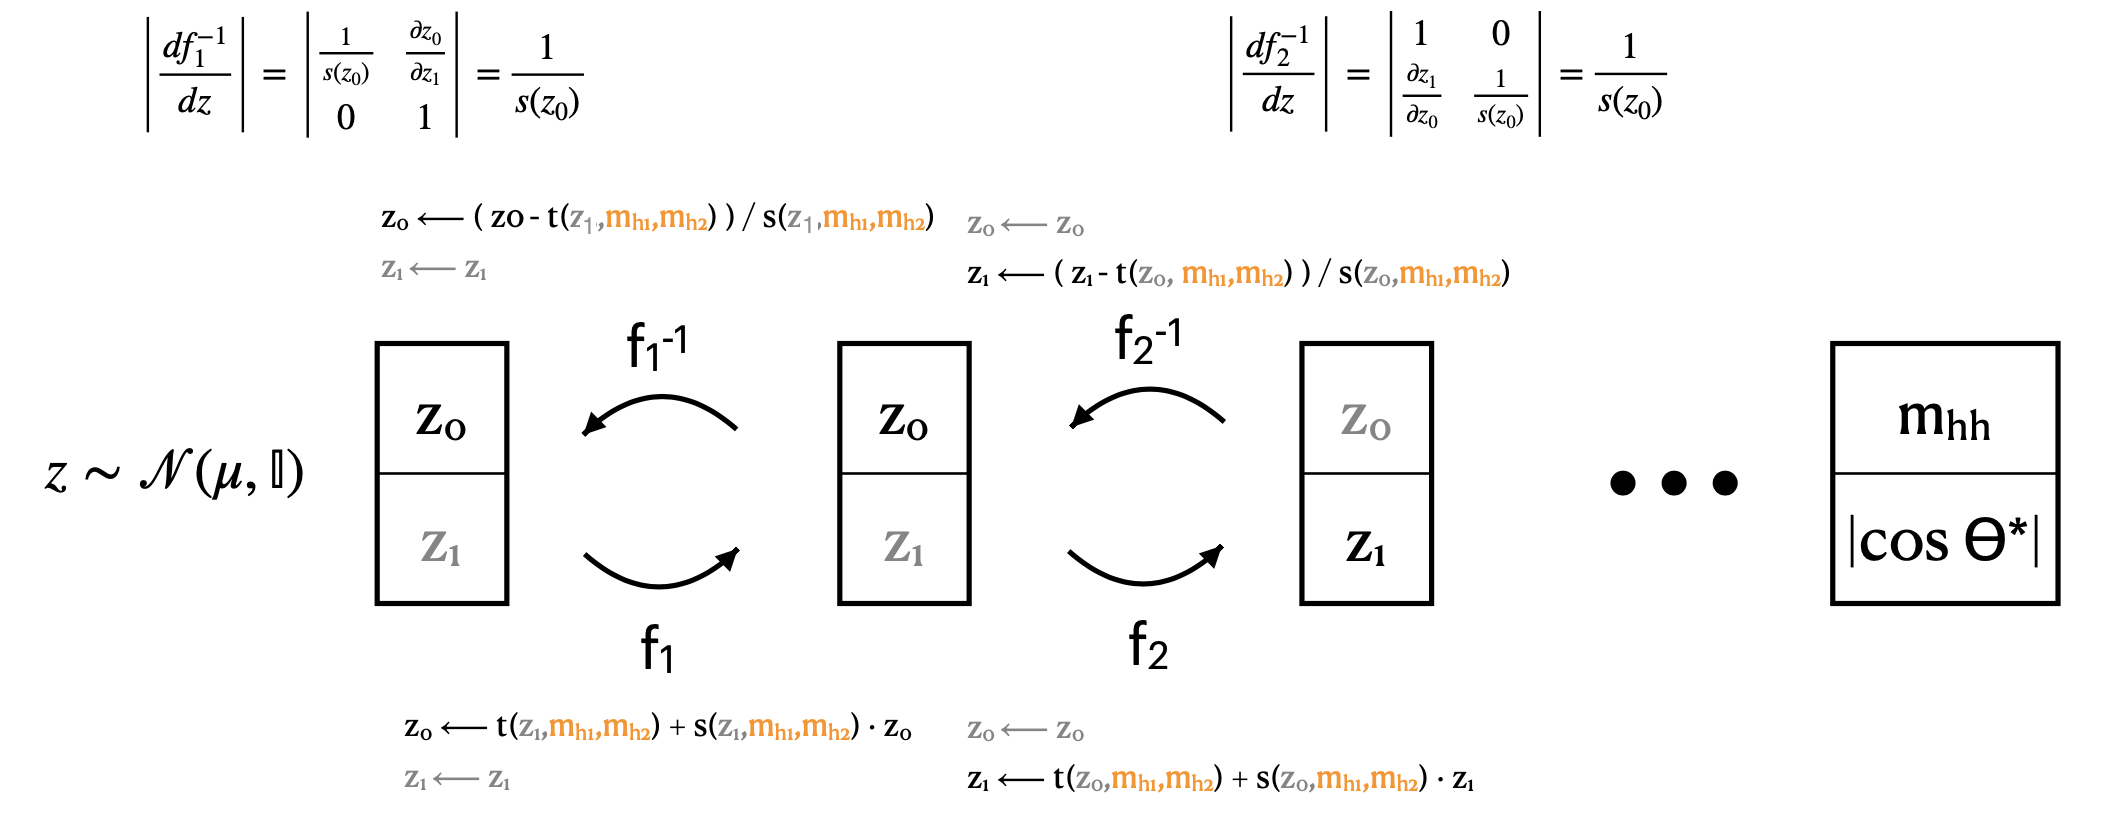
\includegraphics[width=\textwidth]{figures/flows/flow-architectures/Real-NVP-conditional}
    \caption{The extension of the Real-NVP for a conditional 2 variable flow.}
    \label{fig:rnvp-cond}
\end{figure}

\FloatBarrier
\clearpage
\subsection{Neural Spline Flows}

One of the limitations of Real NVPs is their limited expressivity. There is no proof that affine transformations are univeral density approximators.
By replacing the affine (linear) transformations with higher order splines allows more expressivity for modeling more complex densities. \textcolor{red}{Are these universal density approximators? I think the last 2 might be.}
The only constraint needed to ensure the invertibility of $f_i$ is that the $f_i$ are monotonic functions (here, chosen to be increasing functions, as shown in \Fig{\ref{}}.

Let $i$ be the dimension of the transforming variable, and $j$ be the corresponding flow layer.

\textbf{Relevant papers:}
\begin{itemize}
	\item Quadratic spline flow \cite{1808.03856}
	\begin{equation}
		f_j(x_i) = a_{ij} x_i^2 + b-{ij} x_i + c_{ij}
	\end{equation}
	\item Cubic spline flow: \cite{1906.02145}
		\begin{equation}
		f_j(x_i) = a_{ij} x_i^2 + b_{ij} x_i^2 + c_{}ij x_i + d_{ij}
	\end{equation}
	\item Rational quadratic spline flow: \cite{1906.04032}
	\begin{equation}
		f_{jk}(x_i) = \frac{a_{ij} x_i^2 + b_{ij} x_i + c_{ij} } { d_{ij} x_i^2 + e_{ij} x_i + f_{ij}}
	\end{equation}
\end{itemize}

%
%\begin{figure}
%\centering
%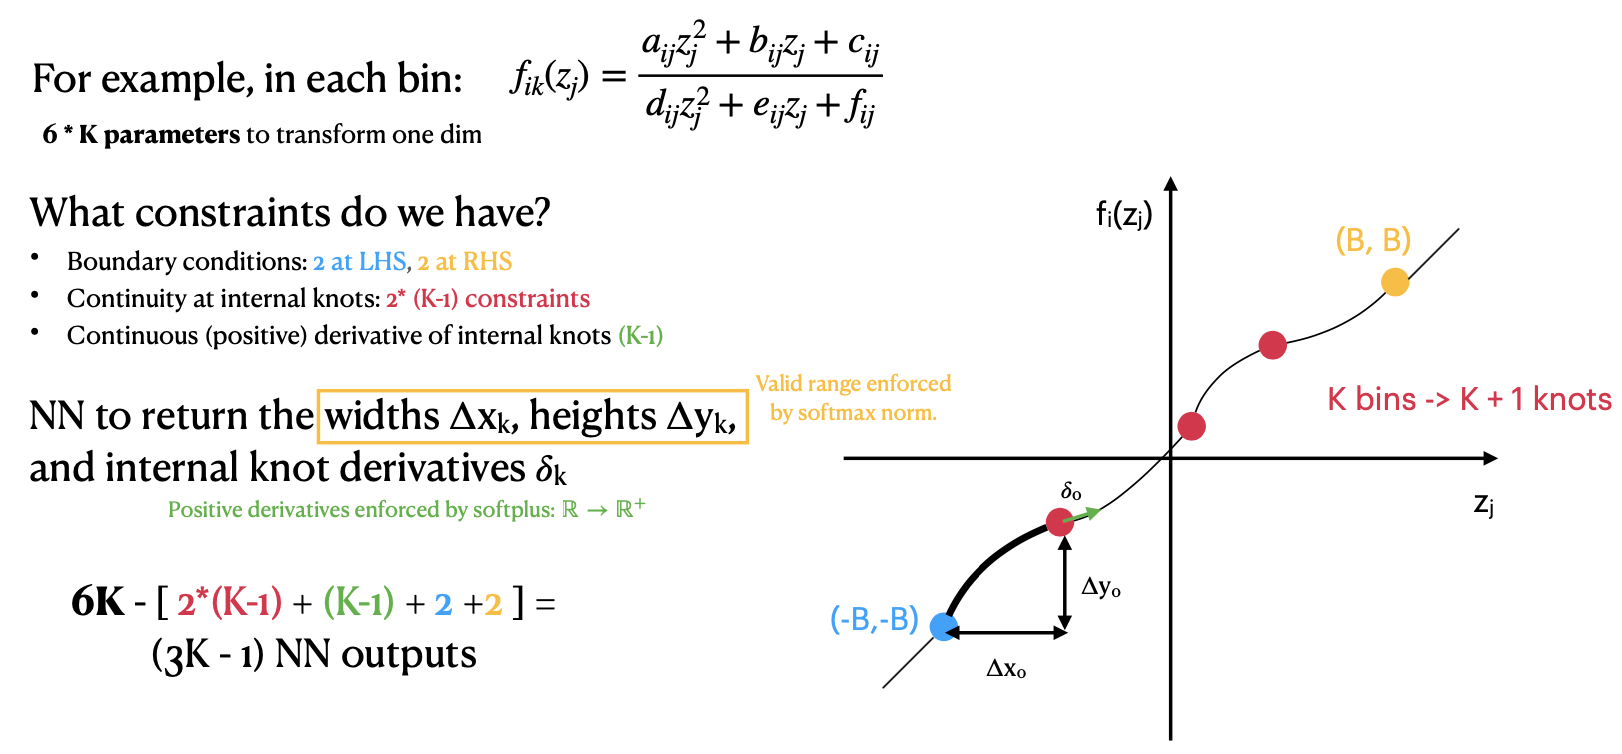
\includegraphics[width=\textwidth]{figures/flow-architectures/nsf-explanation}
%\caption{}
%\label{fig:nsf-explanation}
%\end{figure}
%
%\textcolor{red}{AGH - do I need to be careful about not overloading $f$ to be both a function and a constant? }
%
%TO DO: Summarize \Fig{\ref{nsf-explanation}} in text.
%
%\begin{minipage}{0.5\textwidth}
%Look how Figure looks!
%\begin{figure}
%\centering
%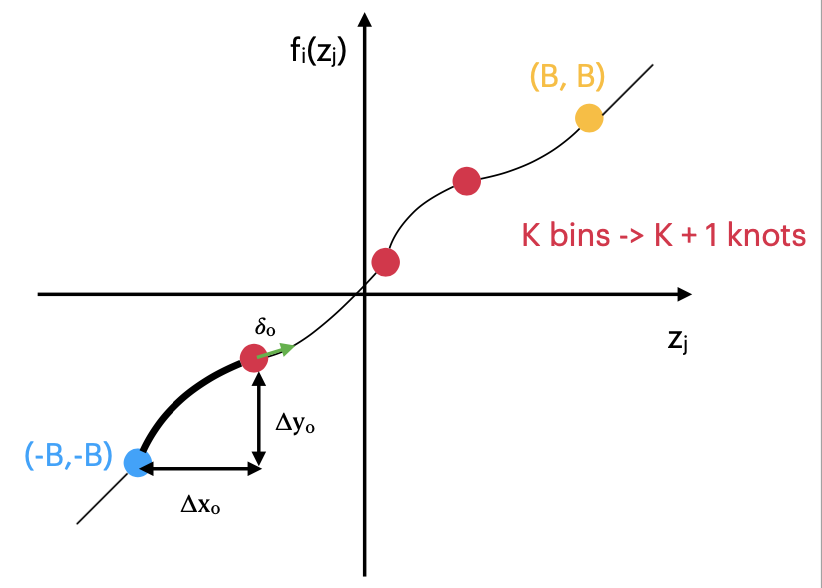
\includegraphics[width=\textwidth]{figures/flow-architectures/nsf-graphic}
%\caption{Graphic explaining the parmetrization for a neural spline flow.}
%\label{fig:nsf-graphic}
%\end{figure}
%\end{minipage}
%
%
%Then instead of taking two sets of variables, this architecture also uses a generalized permutation:
%
%\begin{equation}
%	W = P L U
%\end{equation}
%
%where $P$ is the permutation matrix (to allow for random permutations?), $L$ is a lower triangular matrix, and $U$ is an upper triangular matrix.
%
%This is attractive b/c $det(W)$ only takes $\mathcal{O}(d)$ time to compute (where $d$ is the number of modelling dimensions) and inverting this step involves solving two triangular systems, which is a $\mathcal{O}(d^2)$ operation, the same order as inverting the spline flow operations. (or at least - I think this is what I meant).
%
%These generalized permutaions are also used for the TAn and glow papers - both v strong density estimation baselines.